% Publisher's series page, source PDF page 315.
\chapter*{MIT Press Computer Science Series}
\addcontentsline{toc}{chapter}{MIT Press Computer Science Series}

The MIT Press, with Peter Denning, general consulting editor, and
Brian Randell, European consulting editor, publishes computer science books
in the following series:

\begingroup
\setlength{\parindent}{0pt}
\setlength{\parskip}{0.7\baselineskip}

ACM Doctoral Dissertation Award and Distinguished Dissertation Series

Artificial Intelligence, Patrick Winston and Michael Brady, editors

Charles Babbage Institute Reprint Series for the History of Computing,
Martin Campbell-Kelly, editor

Computer Systems, Herb Schwetman, editor

Exploring with Logo, E. Paul Goldenberg, editor

Foundations of Computing, Michael Garey, editor

History of Computing, I. Bernard Cohen and William Aspray, editors

Information Systems, Michael Lesk, editor

Logic Programming, Ehud Shapiro, editor; Fernando Pereira, Koichi
Furukawa, and D. H. D. Warren, associate editors

The MIT Electrical Engineering and Computer Science Series

Scientific Computation, Dennis Gannon, editor
\par\endgroup

% Source PDF pages 316--319 are blank/library endpapers, loan stamps, and a
% library barcode, not book text. They are not inserted as scanned pages.

% Re-typeset back-cover text from source PDF page 320. Only the author portrait
% is a cropped photograph; the cover text remains selectable/editable text.
\clearpage
\begin{titlepage}
\thispagestyle{empty}
\pagecolor{coverblue}
\color{white}
\sffamily
\small
\setlength{\parindent}{0pt}
\setlength{\parskip}{0.6\baselineskip}

\textbf{The MIT Press}\\
Massachusetts Institute of Technology\\
Cambridge, Massachusetts 02142

\vspace{0.8cm}
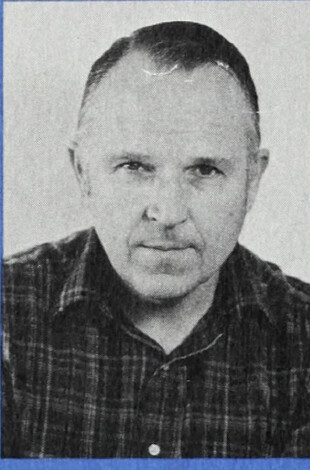
\includegraphics[height=2.4cm]{figures/author-portrait.jpg}

\textbf{Simulating Computer Systems:}\\
Techniques and Tools\\
by M. H. MacDougall

\textit{Simulating Computer Systems} provides an introduction to simulation
for computer and communication-system designers who want to analyze the
performance of their designs. In it MacDougall describes a discrete-event
simulation language called \textbf{smpl}, discusses simulation modeling with
\textbf{smpl} (using a variety of models as examples), describes the design of
\textbf{smpl}, and presents a C language implementation.

The book's first part introduces \textbf{smpl} simulation operations using a
queueing network simulation model; addresses the development, the
verification, and the validation of simulation models (including hybrid
modeling and the use of analytic models in verification); and describes how
to estimate the accuracy of simulation results. A multiprocessor system model
and a CSMA/CD LAN model are studied in detail to emphasize the joint use of
simulation and analytic models and to further illustrate the use of
\textbf{smpl}. Projects for the reader include a CPU pipeline model and a token
ring LAN model.

The implementation of \textbf{smpl} is the focus of the book's second part,
which describes the design of \textbf{smpl} function and data structures and
outlines a variety of extensions. This description, together with the C source
listing provided, will allow the reader to implement \textbf{smpl} on any
system.

M. H. MacDougall is with the Advanced Computer Group at Apple Computer,
where he is involved in the design of high-performance personal computers
for the 1990s. \textit{Simulating Computer Systems} is included in the Computer
Systems series, edited by Herb Schwetman.

\vfill
\hfill\textcolor{black}{MACAH 0-262-13229-X}
\end{titlepage}
\nopagecolor
